\documentclass[11pt,a4paper,oneside]{article}
\usepackage{amsmath,amsthm,amssymb,amsfonts,adjustbox,bm}
%\usepackage[dvipsnames]{xcolor}
\usepackage{mathtools}
\usepackage{refstyle}
\usepackage{pdflscape}
\usepackage[flushleft]{threeparttable}
\usepackage{multirow}
\usepackage{longtable}
\usepackage{eurosym}
\usepackage{enumerate}
\usepackage{booktabs}
\usepackage{siunitx}
\usepackage{rotating}
\usepackage{graphicx}
\usepackage{subcaption}
\usepackage[section]{placeins}
\usepackage{xcolor}
\usepackage{geometry}
\usepackage{changepage}
\usepackage[natbibapa]{apacite}
\newcommand{\footremember}[2]{%
   \footnote{#2}
    \newcounter{#1}
    \setcounter{#1}{\value{footnote}}%
}
\newcommand{\footrecall}[1]{%
    \footnotemark[\value{#1}]%
} 


\usepackage[colorlinks=true, citecolor=blue, linkcolor=blue, urlcolor=blue,breaklinks]{hyperref}


\title{Skills, Inequality, and Referrals \\ \large Preregistration \\}
\author{Jhon Díaz\footnote{Universidad Autónoma de Bucaramanga}, Manuel Munoz\footremember{liser}{Luxembourg Institute of Socio-Economic Research}, Ernesto Reuben\footnote{Division of Social Science, New York University Abu Dhabi} \footrecall{liser}, Reha Tuncer\footnote{University of Luxembourg}}
% \footnote{Center for Behavioral Institutional Design at New York University Abu Dhabi} 
\begin{document}

\maketitle



\section*{Abstract}

Referrals propagate inequality because they are alike in many dimensions, making them problematic for diversity. On the other hand, ties to higher social classes in an individual's network lead to better outcomes (i.e., upward mobility) through the sharing of opportunities. For ties to form, though, simple exposure is not enough: Individuals across social classes should befriend each other to benefit. Universities are potentially one such environment where exposure and friendship among different social classes are plenty. Can quotas change referral choices? And if so, do different skill requirements lead to particular referrals? We conduct an incentivized field experiment in a Colombian university to measure the effects of (i) a low social class quota and (ii) two different skill requirements on referral composition and quality. \medskip \\
\textbf{Keywords:} behavioral economics, referrals, field experiment, skills, inequality, upward mobility


\section{General remarks and background}

In this study, participants perform two skill tests in addition to a referral and a guessing task. The data collection will begin in the last week of April 2024. Institutional Review Board approvals for this study were obtained from NYU Abu Dhabi (HRPP 2024-50) and the University of Luxembourg (ERP 24–028). In this document, we describe the study and the procedures followed to begin data collection.

\section{Data collection and Sample}
\textbf{Data collection.} The data collection will begin on April 22, 2024. Our local partner at Universidad Autónoma de Bucaramanga (UNAB), the Social Bee Lab, organized scheduled visits for classrooms and recruited research assistants to administer the study protocol. Students attending class on the scheduled visit dates are invited to participate in the study. Each classroom comprises a separate data collection session. The expected duration of each session is 20 minutes. Participants will use their smartphones to access the Qualtrics survey during sessions. We have no reason to expect delays in the data collection. Visiting all the classrooms will take one week, and data collection will be completed by May 2024.\medskip \\
\textbf{Sample.} 864 undergraduate students enrolled at UNAB (Bucaramanga, Colombia) are invited to join the study. The students are spread across 36 classrooms, and their ages vary between 17 and 30. We achieved the maximum feasible sample size given the available participants. Our final sample will consist of the students who both consent to participate and complete the study protocol.

\section{Variables}

\subsection{General Description}
The study begins with a demographic survey. The rest of the study is divided into three parts. Participants perform various experimental tasks designed to obtain behavioral measures in each part. Participants’ choices in these tasks are incentivized and determine their bonus earnings. In addition to the demographic survey and behavioral measures, UNAB provides complementary administrative data.

\subsection{Demographic Survey Questions}
\textbf{Gender.} We ask participants: ``What is your gender?" Answer options: Man, Woman.\medskip \\
\textbf{Stratum.} We ask participants: ``What is the socio-economic stratum to which your family belongs?" Answer options range from 1 to 6. This is a government-assigned number assigned to every household in Colombia based on neighborhood-level wealth. It's a widely recognized classification system that directly affects utility costs and is visible on all utility bills. It categorizes neighborhoods into six strata, from 1 (lowest socioeconomic status) to 6 (highest socioeconomic status). Residents in higher strata pay more for utilities, while those in lower strata receive subsidies.\medskip \\
\textbf{Parental Education.} We ask participants: ``What is the highest level of education acquired by your father (mother)?" Answer options are: Primary school, High school, Technical school, Undergraduate, Graduate, Postgraduate, Not applicable.

\subsection{Administrative Data}
\textbf{Co-enrollment History.} UNAB provides the co-enrollment history of participants in this study. This is a detailed list of all the classes participants have taken since their enrollment at the university, the semester during which they have taken these classes, and the classroom in which they have taken them.  \medskip \\
\textbf{GPA.} UNAB provides the transcripts of the classes participants have taken since their enrollment at the university. \medskip\\
\textbf{National University Entry Exam.} UNAB provides participants' scores in the national-level university entry exam that every student passes before beginning their studies in a Colombian higher education institution. \medskip\\
\textbf{Study Program.} UNAB provides the study track of participants. \medskip\\
\textbf{Age.} UNAB provides the age of participants.

\subsection{Incentivized Measures}
\subsubsection{Skill Assesment}
Participants complete two incentivized skill assessment tests in the first part of the study. The tests are presented in a randomized order. Due to time constraints, participants have 5 minutes for each test. \medskip\\
\textbf{Incentives.} The incentives for performance in this part are as follows. 10\% of participants in each classroom (rounded upwards) are randomly selected for a lottery to win a bonus worth 100,000 Pesos (about \$26). We will randomly select one test for each lottery participant and draw a number between 1 and 100. If the percentage of correct answers in the test exceeds the number, the participant receives the bonus. \medskip\\
\textbf{Cognitive Skills.} We use Raven's Progressive Matrices to measure cognitive skills \citep{raven_performances_1936, raven_standard_1976}. Raven’s test is a well-established measure of fluid intelligence, i.e., an individual’s capacity to reason and solve problems in novel situations independent of past knowledge \citep{schilbach_psychological_2016}. We use an 18-item version featuring increasingly difficult pattern-matching questions, with 6 answer choices for the first 9 items and 8 choices thereafter. After reading the test instructions and going through an example, participants complete the 18 matrices. Participants see one matrix per screen. They do not have the option to return to previous screens but can continue to the next screen without answering. We do not provide feedback on performance to the participants. Chances to earn financial compensation increase with each correctly solved matrix by 5.5\% (=1/18), conditional on this test being selected for the lottery.   
\medskip\\
\textbf{Social Skills.} We measure social skills with the Multiracial Reading the Mind in the Eyes Test (MRMET) from \citet{kim_multiracial_2022}. Based on the original RMET \citep{baron-cohen_reading_2001}, the MRMET is a more race- and gender-inclusive test measuring the ability to recognize emotions in others. The test has been previously used in economic experiments \citep{van_leeuwen_predictably_2018, weidmann_team_2021}. We use the first 36 (out of 37) items in MRMET. The test consists of cropped photos of faces, with only the eye region visible. In each photo, a professional actor portrays an emotion. Participants choose the emotion that best describes the photo from four answer choices. After reading the test instructions and completing an example, participants go through 36 photos. Participants see one photo per screen. They do not have the option to return to previous screens but can continue to the next screen without answering. We do not provide feedback on performance to the participants. Chances to earn financial compensation increase with each correctly found emotion by 2.78\% (=1/36), conditional on this test being selected for the lottery.


\subsubsection{Referral Task} \label{referral_task}
In part two, participants make referrals based on the predicted performance of their classmates. They pick three classmates with the highest predicted scores for each skill assessment test. The referral tasks for skills are presented in a randomized order, and they are not timed. \medskip\\
\textbf{Top 3.} To incentivize referrals by performance, we introduce a classroom-level ranking system. We rank participants by the number of correct answers for both skill measures. The three highest-scoring classmates designate the top 3 performers for a skill. In case of a tie for a spot among the top 3 performers, we will randomly select the top 3 participants to ensure fairness when multiple participants have the same score.\medskip\\
\textbf{Incentives.} Incentives are set for making high-performing referrals in this part. 20\% of participants in each classroom (rounded upwards) are randomly selected for a lottery to win a bonus worth 100,000 Pesos (about \$26). We will randomly select one test and one referral for each lottery participant. The participant receives the bonus if the selected participant is among the top 3 performers for that skill. \medskip\\
\textbf{Referral Choices.} Referrals can only be made among other classmates. Self-referrals are not allowed. Referrals can be made to the same three individuals twice. Participants see a list with the names of their classmates and tick the box in front of a name for their referral choice. 

\subsubsection{Guessing Task}\label{guessing_task}
In part three, participants make guesses based on the predicted social class of their classmates. This measures their ability to distinguish social class independent of performance expectations. Participants pick three classmates they predict to be among the lower social classes designated by strata 1 to 3. The guessing task is not timed. \medskip\\
\textbf{Incentives.} The incentives for performance in this part are as follows. 10\% of participants in each classroom (rounded upwards) are randomly selected for a lottery to win a bonus worth 100,000 Pesos (about \$26). We will randomly select one guess for each lottery participant. The participant receives the bonus if the selected guess is a lower social class individual designated by strata 1 to 3. \medskip\\
\textbf{Social Class Guesses.} Guesses can only be made among other classmates. Participants see a list with the names of their classmates and tick the box in front of a name for their guess.
\subsubsection{Unincentivized Belief Elicitation}
Participants are asked to predict their performance in the two assessment tests used to measure cognitive and social skills. After passing each test, they make a single unincentivized prediction about the relative frequency of participants who perform worse than them.\medskip\\
\textbf{Cognitive Skills.} We ask: ``If we randomly choose 10 participants from this classroom, how many people do you think solved fewer correct problems than you?''. Answer options range from 0 to 10; participants use a slider to respond.\medskip\\
\textbf{Social Skills.} We ask: ``If we randomly selected 10 participants from this classroom, how many people do you think solved fewer correct pictures than you?''. Answer options range from 0 to 10; participants use a slider to respond.

\subsubsection{Skills Report}
\textbf{Feedback Decision.} This question comes at the end of the study. We ask participants: ``Do you want to know your scores on the general intelligence test and the social skills test? We can analyze the data and give you a report that explains your strengths in these two areas. Also, what these strengths mean and how you can leverage them for personal and professional development." We also inform participants that they will be contacted for further studies if they consent. Answer options are: ``I can be contacted for new studies and to send me my report.'', ``I can be contacted to send my report, but not for new studies." ``No, I do not want to be contacted again." We collect the student email addresses of participants who agree to be contacted in the future.

\section{Experimental Conditions}
This study follows a 2x2 factorial design, with two within- and two between-subjects conditions. \medskip\\
\textbf{Within-subjects.} All participants complete the referral task (section \ref{referral_task}) followed by the guessing task (section \ref{guessing_task}). These two tasks represent the within-subjects conditions of this study. \medskip\\
\textbf{Between-subjects.} Participants are randomized into baseline and quota conditions balancing gender and social class in each classroom. These conditions only impact the selection procedure for the top 3 performers in the referral task (section \ref{referral_task}). The baseline condition is described above and remains the same: We rank participants by the number of correct answers for both skill measures in every classroom, and the three highest-scoring classmates designate the top 3 performers for a skill, regardless of other characteristics. The quota condition ensures at least one lower social class participant makes it into the top 3. It imposes the following changes: The highest-scoring lower individual takes the first spot in the top 3. The remaining places are assigned without regard to social class. Ties among the top 3 are solved randomly, as described previously.

% \begin{table}[]
% \centering
% \begin{tabular}{lll}
%                                        & \textbf{Baseline}     & \textbf{Quota}        \\ \cline{2-3} 
% \multicolumn{1}{l|}{\textbf{Referral}} & \multicolumn{1}{l|}{} & \multicolumn{1}{l|}{} \\ \cline{2-3} 
% \multicolumn{1}{l|}{\textbf{Guessing}} & \multicolumn{1}{l|}{} & \multicolumn{1}{l|}{} \\ \cline{2-3} 
% \end{tabular}
% \caption{2x2 factorial design}
% \label{tab1}
% \end{table}


\section{Analyses}

\subsection{Main Analysis: Social class and referral choices at baseline}
We will start our analysis by examining whether belonging to the same social class predicts referral choices. In a world without bias, we should expect participants to refer based only on performance, regardless of their own and their referral's social class. In contrast, past evidence suggests we should expect homophily \citep{beaman_job_2018,bolte_role_2021, montgomery_social_1991}. Do different social classes refer to the extent of what their referrals' performance suggests?\\

\noindent\textbf{Hypothesis 1 - Social class bias}\\
\noindent\textbf{H1a.} Does the probability of being referred depend on the social class of the potential nominees after controlling for their performance and the social class composition at the session level? In other words, is there social class bias in referrals?\\
\noindent\textbf{H1b.} Which social group makes more referrals to their own social class, controlling for performance and the social class composition at the session level? Do the lower or higher social class individuals drive the bias?

\subsection{Main Analysis: Social class and referral choices across conditions}
We then examine whether the quota condition causes changes in referral compositions regarding social classes. We are also interested in understanding the equity-efficiency tradeoff of quotas, if there is one. Specifically:\\

\noindent\textbf{Hypothesis 2 - Social class quota}\\
\noindent\textbf{H2a.} Does the quota cause an increase in the number of lower social class referrals, controlling for the social class composition at the session level?  \\
\noindent\textbf{H2b.} Does the quota cause a decrease in referral quality, controlling for the social class composition at the session level? \\
\noindent\textbf{H2c.} Does the impact of the quota on referral quality and the number of lower social class referrals depend on whether the referrals are for cognitive or social skills?

\subsection{Main Analysis: Mechanisms driving bias}
We will start by looking at referral performance. Experimental evidence has shown that referrals from high-performing individuals perform better in tasks than others \citep{beaman_who_2012, beaman_job_2018,pallais_why_2016}. More precisely:\\

\noindent\textbf{Hypothesis 3 - Referrer Performance}\\
\noindent\textbf{H3a.} Do referrers with higher cognitive and/or social skills make higher quality referrals?  \\
\noindent\textbf{H3b.} Do referrers with higher cognitive and/or social skills have a smaller social class bias when making referrals?

\subsection{Exploratory Analysis}
We examine the remaining variables to complement the findings for our primary research questions. What other types of homophily do we observe in our sample? How does the referrer-referral performance correlation depend on other characteristics?     \\

\noindent\textbf{Hypothesis 4 - Additional Variables}\\
\noindent\textbf{H4a.} Does the probability of being referred depend on other characteristics of the potential nominees (e.g., age, GPA, national university entry exam score, parental education, gender, co-enrollment history, ...), controlling for performance and these characteristics at the session level? \\
\noindent\textbf{Hba.} Does the quality of referrals depend on other characteristics of the referrer (e.g., age, parental education, GPA, time spent at the university,...)? \\

\bibliographystyle{apacite}
\bibliography{referrals}

\appendix
\section{Experimental Protocol}
We include the English version of the experimental protocol used in Qualtrics. Participants saw the Spanish version. Horizontal lines indicate page breaks, and clarifying comments are inside brackets.

\noindent\rule{\textwidth}{0.4pt}\\

\noindent Please enter the password:

\noindent [classroom-specific password sent the day before data collection]

\noindent\rule{\textwidth}{0.4pt} \\

\noindent\textbf{Welcome}\\

\noindent Welcome to this study organized by the Social Bee Lab. You have been invited to participate in a survey where you can make a series of decisions. The study takes approximately 20 minutes to complete. During the study, you should not communicate with any other students. If you have any questions at any time, please raise your hand. One of the assistants will help you privately. \\

\noindent In this study, you can win bonus money depending on your choices. In total, we will draw [classroom-specific number equal to 40\% of class size] bonuses of 100.000 pesos among the participants of this classroom. It is also possible for the same person to win more than one voucher. The following screens will detail how the bonus draw will be conducted. The UNAB finance office will make the payment of the vouchers through Nequi.\\

\noindent All your decisions in this survey will be anonymized. Therefore, the answers you provide will not affect your grades in this class or your records at the university. We will use your personal information to determine the bonus allocation, but after that, we will remove any data that identifies you. \\

\noindent This survey has several parts. Each of these parts has specific instructions. Please read the instructions for each part carefully because they describe how you can earn bonuses. This study has been approved by the Ethics Committee of New York University Abu Dhabi (NYU Abu Dhabi) on the condition that all the information we provide is true and all the bonuses we offer are real.\\

\noindent On the next screen, we present you with an informed consent form that you must accept to participate in this study.

\noindent\rule{\textwidth}{0.4pt}\\

\noindent \textbf{Informed Consent} \\ 

\noindent You have been invited to participate in a study to learn more about how people make decisions in common scenarios. \\

\noindent  This study is conducted by Professor Ernesto Reuben of New York University in Abu Dhabi and the Social Bee Lab at UNAB. The purpose of this study is to broaden our understanding of how people make decisions. \\

\noindent  Participation in this study is voluntary. You may opt-out at any time. No known risks are associated with your participation in this project beyond those of everyday life. Apart from the monetary bonuses that will be drawn, participation has no direct benefits.\\

\noindent  The Social Bee Lab is in charge of data collection. Your answers in this study are anonymous and will not be shared with anyone. In addition to your answers, UNAB will provide the Social Bee Lab with administrative records of your courses and your university entrance exam score. Your records, decisions, and your identity will be kept strictly confidential. Data about you collected within the scope of the study are used for scientific purposes only and are treated as strictly confidential. The Social Bee Lab will anonymize your data, and the researcher will analyze it without knowing your identity. All data generated will be stored on the researcher's computer. You have the right to access your personal data and request its deletion. You can exercise this right by contacting the researcher.\\

\noindent  If something is unclear or you have any questions, you can contact Dr. Manuel Muñoz Herrera at manuel.munoz@liser.lu.\\

\noindent  If you have questions about your rights as a participant, you can contact the NYUAD IRB office at IRBnyuad@nyu.edu.\\

\noindent  By continuing to the next screen, you agree to participate in this study.\\

\noindent\rule{\textwidth}{0.4pt}\\

\noindent Before you start, please answer these four questions. \\

\noindent What is your gender? \\ 

\noindent [Male, Female] \\

\noindent What is the socio-economic stratum to which your family belongs? \\

\noindent [Stratum 1 to Stratum 6] \\

\noindent What is your father's highest acquired level of education?\\

\noindent [Primary school, High school, Technical school, Undergraduate, Graduate, Postgraduate, Not applicable.] \\

\noindent What is your mother's highest acquired level of education?\\

\noindent [Primary school, High school, Technical school, Undergraduate, Graduate, Postgraduate, Not applicable.] \\

\noindent\rule{\textwidth}{0.4pt}\\

\noindent \textbf{Part 1} \\

\noindent You will now participate in two quizzes, each lasting five minutes. Please try to answer them to the best of your ability. \\

\noindent We will allocate up to [classroom-specific number equal to 10\% of class size] bonuses of 100.000 pesos in this first part. The steps to allocate the bonuses for Part 1 are explained below.\\

\noindent\rule{\textwidth}{0.4pt}\\

\noindent [classroom-specific illustrations explaining the incentive structure] \\

\noindent\rule{\textwidth}{0.4pt}\\

\noindent [random assignment to either cognitive or social skills test] \\

\noindent \textbf{Test - Cognitive Skill}\\

\noindent In this test, you will see a series of images. Below is an example of the images you will solve. At the top of each image, there is a pattern with a piece that has been removed. Your task is to choose which of the six pieces completes the pattern correctly. For each image, there is only one correct piece. Look at the following example: \\

\begin{figure}[htbp]
  \centering
  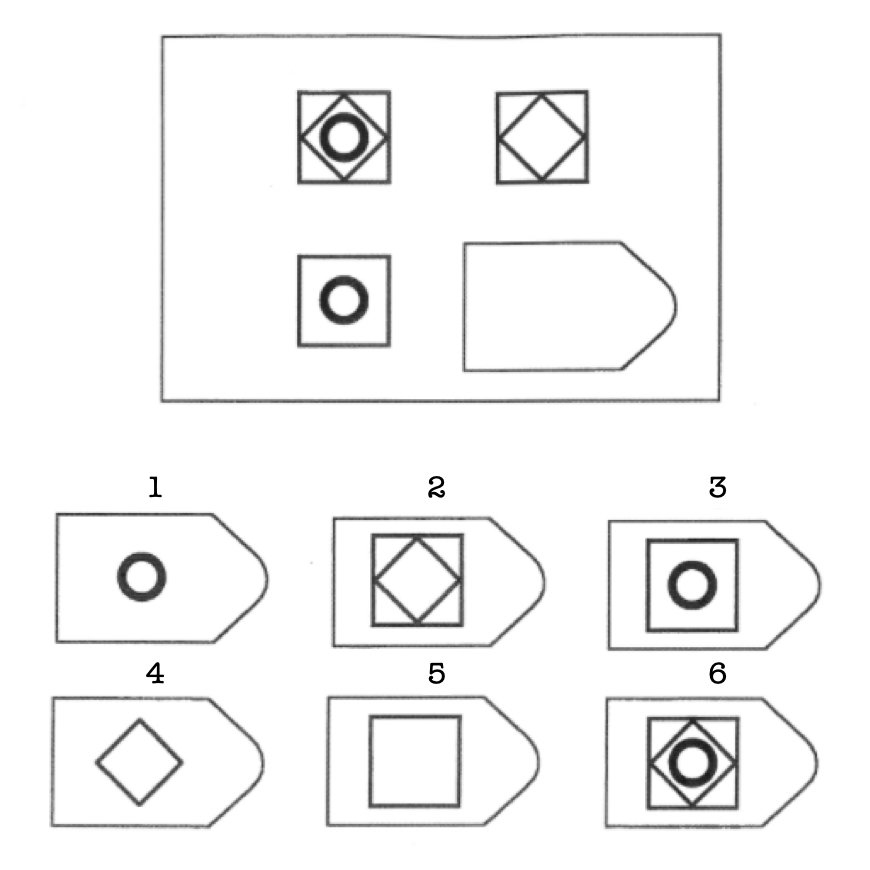
\includegraphics[scale=0.2]{Ravens Survey.jpg}
\end{figure}

\noindent First, notice a square in the upper left, the upper right, and the lower left. Also, notice that the circle is eliminated when one moves from the upper left to the upper right. Finally, the rhombus is eliminated when moving from the upper left to the lower left. Therefore, the correct piece should eliminate the circle and the rhombus, leaving only a square. So, the correct answer is piece 5. \\

\noindent To give your answer to each image, you must choose the correct option and then continue to the next screen. After giving your answer you cannot go back. \\

\noindent You will have 5 minutes to complete the test, which consists of 18 images to solve. The percentage of correct answers will determine your chances of winning one of the 100.000 pesos bonuses if you are chosen for the drawing. \\

\noindent\rule{\textwidth}{0.4pt}\\

\noindent Are you ready? \\
 
\noindent Your 5 minutes will start as soon as you move to the next screen. \\

\noindent\rule{\textwidth}{0.4pt}\\

\noindent \textbf{Problem 1}\\

\noindent [screenshot of Raven's matrix] \\

\noindent [After participants submit an answer, a new matrix appears on the screen. The sequence of matrices is the same for all participants. Participants cannot return to a previous screen. Participants do not have to provide answers for all 18 matrices.] \\

\noindent\rule{\textwidth}{0.4pt}\\

\noindent You have finished the test. You can proceed to the next screen. \\

\noindent\rule{\textwidth}{0.4pt}\\

\noindent \textbf{How did you do on the test?} \\

\noindent If we randomly choose 10 participants from this classroom, how many people do you think solved fewer correct problems than you?\\

\noindent [Slider from 0 to 10]\\

\noindent\rule{\textwidth}{0.4pt}\\

\noindent \textbf{Test - Emotions} \\
 
\noindent In this test, you will see a series of photographs. Below is an example of the pictures you will see. In each picture, you will see the eyes of a person. Below the picture, you will see four possible emotions that this person is feeling. Your task is to choose which of the four emotions correctly describes what the person is feeling. For each picture, there is only one emotion. Look at the following example: \\

\begin{figure}[htbp]
  \centering
  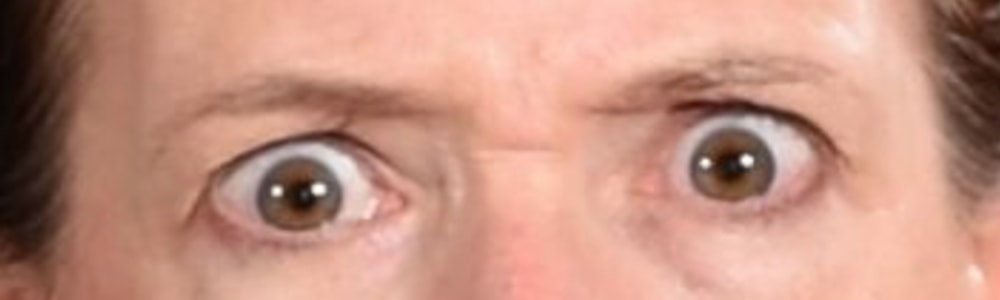
\includegraphics[scale=0.2]{3Aghast-J.jpg}
\end{figure}

\noindent [Happy, Disappointed, Shocked, Worried] \\

\noindent In this case, the correct answer is: Shocked. \\

\noindent To give your answer to each picture, you must choose the correct option and then continue to the next screen. After giving your answer you will not be able to go back. \\

\noindent You will have 5 minutes to complete the test, which consists of 36 photographs to solve. The percentage of correct answers you get will determine your chances of winning one of the 100.000 pesos bonuses if you are chosen for the drawing. \\

\noindent\rule{\textwidth}{0.4pt}\\

\noindent Are you ready? \\
 
\noindent Your 5 minutes will start as soon as you move to the next screen. \\

\noindent\rule{\textwidth}{0.4pt}\\

\noindent \textbf{Photograph 1: Choose the word that best describes the photograph} \\

\noindent [photo from Multiracial Reading the Mind in the Eyes Test] \\

\noindent [After participants submit an answer, a new photo appears on the screen. The sequence of photos is the same for all participants. Participants cannot return to a previous screen. Participants do not have to provide answers for all 36 photos.] \\

\noindent\rule{\textwidth}{0.4pt}\\

\noindent You have finished the test. You can proceed to the next screen. \\

\noindent\rule{\textwidth}{0.4pt}\\

\noindent \textbf{How did you do on the test?} \\

\noindent If we randomly choose 10 participants from this classroom, how many people do you think solved fewer correct photographs than you?\\

\noindent [Slider from 0 to 10]\\

\noindent\rule{\textwidth}{0.4pt}\\

\noindent \textbf{Part 2} \\
 
\noindent At the beginning of this study, all participants took two tests, one on cognitive ability and one on emotions. In this part, we will ask you to recommend the people who in your opinion will score the best on each test. \\

\noindent You may recommend 3 people per test, but you may not recommend yourself. \\

\noindent We will allocate up to [classroom-specific number equal to 20\% of class size] bonuses of 100.000 pesos for Part 2. The steps for allocating bonuses are explained below. \\

\noindent\rule{\textwidth}{0.4pt}\\

\noindent [random assignment to either quota or baseline condition] \\

\noindent [classroom-specific illustrations explaining the incentive structure depending on assignment to either baseline or quota conditions] \\

\noindent\rule{\textwidth}{0.4pt}\\

\noindent [random assignment to either cognitive or social skills referral task] \\

\noindent \textbf{Recommendation - Cognitive Skill}\\

\noindent All participants took a test to identify the missing pattern in each image, as in the example below. This test is used to measure general intelligence.\\

\begin{figure}[htbp]
  \centering
  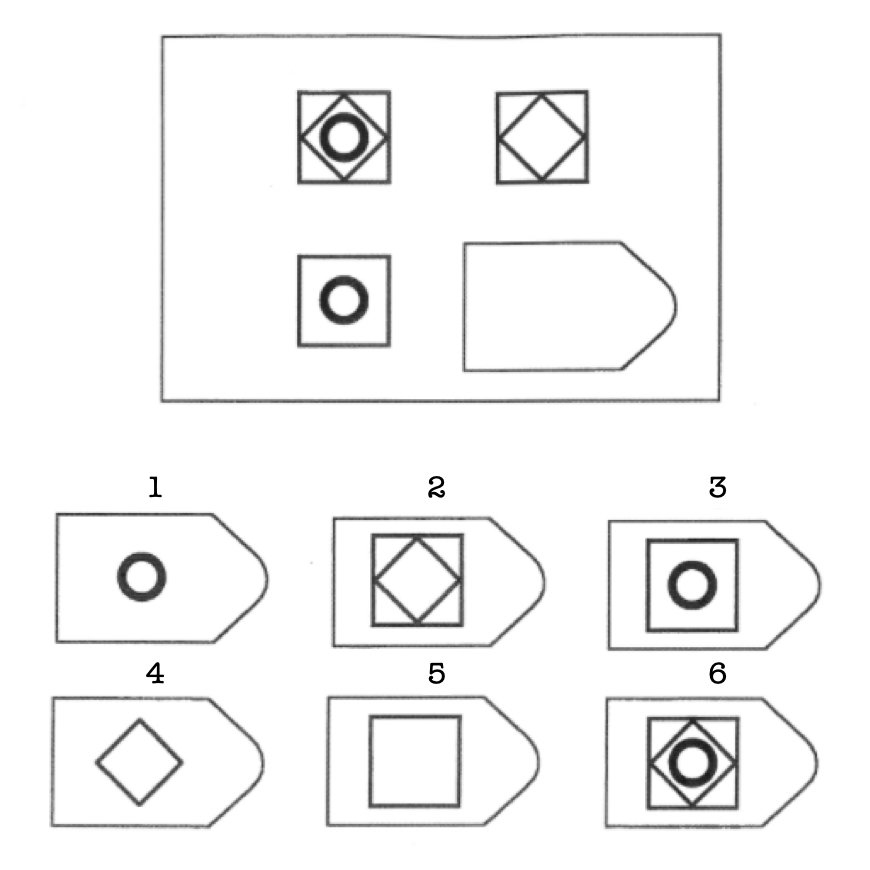
\includegraphics[scale=0.2]{Ravens Survey.jpg}
\end{figure}

\noindent Next, we will present you with a list of the names of all the students in this room. We will ask you to recommend the three people you think will score the highest on the general intelligence test. \\

\noindent If you are chosen by the computer, each of your recommendations in the top 3 increases your chances of winning one of the 100.000 pesos bonuses. \\

\noindent\rule{\textwidth}{0.4pt}\\

\noindent Select the students in this classroom who you consider to have the highest scores on the general intelligence test. (Select 3 students) \\

\noindent [Classroom-specific list of all classmate names visible on one screen. Participants have to pick 3 classmates to continue. Picking their own name invalidates their choices.]\\

\noindent\rule{\textwidth}{0.4pt}\\

\noindent \textbf{Recommendation - Emotions} \\

\noindent All participants took a test where they had to identify the emotion that best described the expression of each image as in the example below. This test is used to measure social skills. \\

\begin{figure}[htbp]
  \centering
  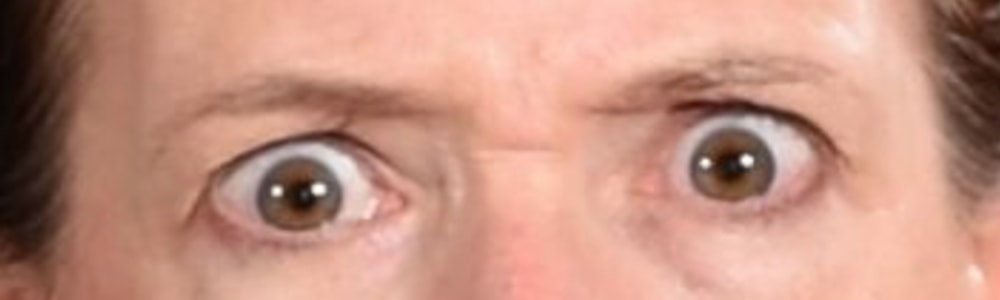
\includegraphics[scale=0.2]{3Aghast-J.jpg}
\end{figure}

\noindent Next, we will present you with a list of the names of all the students in this room. We will ask you to recommend 3 people you think will score the highest on the social skills test. \\

\noindent If you are chosen by the computer, each of your recommendations in the top 3 increases your chances of winning one of the 100.000 pesos bonuses. \\

\noindent\rule{\textwidth}{0.4pt}\\

\noindent Select the students in this classroom who you consider to have the highest scores on the social skills test. (Select 3 students) \\

\noindent [Classroom-specific list of all the names visible on one screen. Participants have to pick 3 classmates to continue. Picking their own name invalidates their choices.]\\

\noindent\rule{\textwidth}{0.4pt}\\

\noindent\textbf{Part 3: Recommendation - Random draw}

\noindent In this part, the computer will randomly choose three students who belong to strata 1, 2, or 3. We will ask you to nominate three people you think the computer will choose. \\

\noindent We will allocate up to [classroom-specific number equal to 10\% of class size] bonuses of 100.000 pesos for Part 3. The steps for allocating the bonuses are explained below. \\

\noindent\rule{\textwidth}{0.4pt}\\

\noindent [classroom-specific illustrations explaining the incentive structure] \\

\noindent\rule{\textwidth}{0.4pt}\\

\noindent Select the students in this classroom who belong to strata 1, 2, or 3, who you think will be randomly selected by the computer (Select 3 students). \\

\noindent [Classroom-specific list of all the names visible on one screen. Participants have to pick 3 classmates to continue. Picking their own name invalidates their choices.]\\

\noindent\rule{\textwidth}{0.4pt}\\

\noindent \textbf{Part 4}

\noindent Do you want to know your scores on the general intelligence test and the social skills test? We can analyze the data and give you a report that explains your strengths in these two areas. Also, what do these strengths mean, and how can you leverage them for your personal and professional development? \\

\noindent If you want to receive your skills report, we need to contact you again. We also want to be able to invite you to new studies where you can participate for more bonus money. Please indicate if you agree to be contacted again. \\

\noindent [I can be contacted for new studies and to send me my report. I can be contacted to send my report, but not for new studies.  No, I do not want to be contacted again.]

\noindent\rule{\textwidth}{0.4pt}\\

\noindent [if participant gives consent to be contacted again] \\

\noindent Please enter your contact email: \\

\noindent [student email]\\

\end{document}
